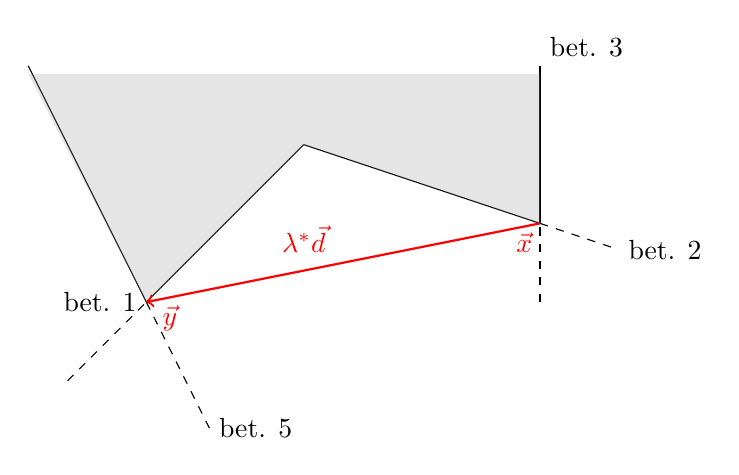
\begin{tikzpicture}[ latex
  s/.style={width=0}]

  %ligning 1
	\draw[domain=-1:0,variable=\x,dashed] 	plot({\x},{\x})  node[left] {bet. 1};
	\draw[domain=0:2,variable=\x] 			plot({\x},{\x});

	
  %ligning 2
	\draw[domain=2:5,variable=\x] 			plot({\x},{-(1/3)*\x+8/3});
	\draw[domain=5:6,variable=\x,dashed] 	plot({\x},{-(1/3)*\x+8/3}) node[right] {bet. 2};
	

  %ligning 3
	\draw[domain=0:1,variable=\y, dashed] 			plot({5},{\y});
	\draw[domain=1:3,variable=\y] 	plot({5},{\y}) node[above right] {bet. 3};
	

	
  %ligning 5
  	\draw[domain=-1.5:0,variable=\x] 	plot({\x},{-2*\x}) ;
	\draw[domain=-0:4/5,variable=\x, dashed] 			plot({\x},{-2*\x}) node[right] {bet. 5} ;


  %løsningsmængden skraveret
	\fill[gray!80,nearly transparent]  (0,0) -- (2,2) -- (5,1) -- (5,2.9) --(-1.5,2.9) --  cycle;
	
  % vektor x
  \node[thick, color=red] (x) at (4.8,0.75) {$\vec{x}$};
  
\node[thick, color=red] (y) at (0.3,-0.2) {$\vec{y}$};
%   %\node[s] (d) at (2, -0.5);
 \draw[thick, color=red, ->](5,1) -- (0,0) node[above, yshift=0.5 cm, xshift=2 cm] {$\lambda^* \vec{d}$} ;
%   \node[] (x) at (2.1, -0.6) {$\vec{x}+\lambda^* \vec{d}$};
%  % \path (x) edge node[right] {$\vec{x}+\lambda^* \vec{d}$} (d) ;
 
\end{tikzpicture}